\documentclass[../ro-fa-lab.tex]{subfiles}
\usepackage{hyperref}
\hypersetup{
    pdftitle={(RO) L9 - Tutorial},   % The title shown in the browser tab
    pdfauthor={},         % Your name or organization
    pdfsubject={},   % A brief description
    pdfkeywords={}
}

\begin{document}

\section{\texorpdfstring{\textbf{Tema Nr. 9: Tutorial}}{Tema Nr. 9: Tutorial}}\label{assign9}


\subsection{Configurare Proiect Visual Studio}\label{visual-studio-project-setup}

\begin{enumerate}
\def\labelenumi{\arabic{enumi}.}
\item
  Accesați Moodle și selectați una dintre următoarele:
\end{enumerate}

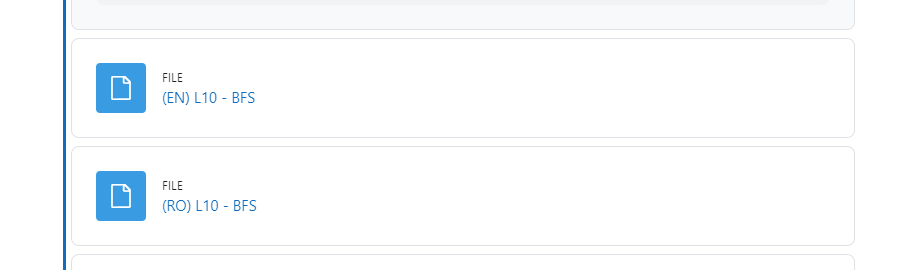
\includegraphics[width=\textwidth,alt={A white rectangular object with a black border Description automatically generated with medium confidence}]{./Resources/tutorial_lab9/image1.png}

Aceasta va rezulta în descărcarea unui fișier `.zip'.

\begin{enumerate}
\def\labelenumi{\arabic{enumi}.}
\setcounter{enumi}{1}
\item
  Creați un Proiect C++ Gol și făcând clic dreapta pe proiect (nu pe soluție) veți putea selecta `Deschideți folderul în File Explorer'.
\end{enumerate}

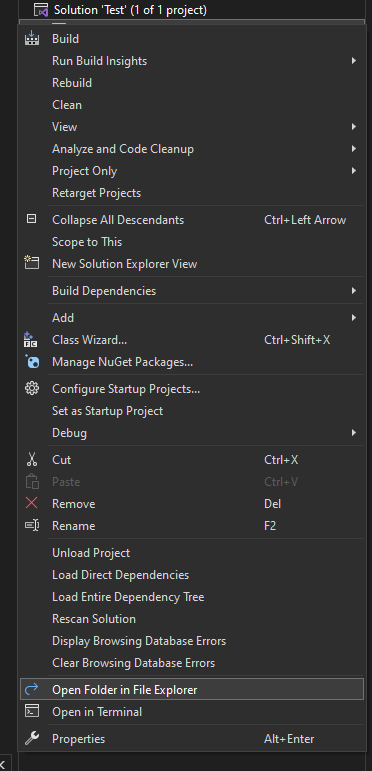
\includegraphics[width=\textwidth,alt={A screenshot of a computer Description automatically generated}]{./Resources/tutorial_lab9/image2.png}

\begin{enumerate}
\def\labelenumi{\arabic{enumi}.}
\setcounter{enumi}{2}
\item
  În acest moment, se va deschide o fereastră `File Explorer'. Deschideți o altă fereastră `File Explorer' la locația descărcărilor dvs. (cel mai probabil folderul Downloads).
\end{enumerate}

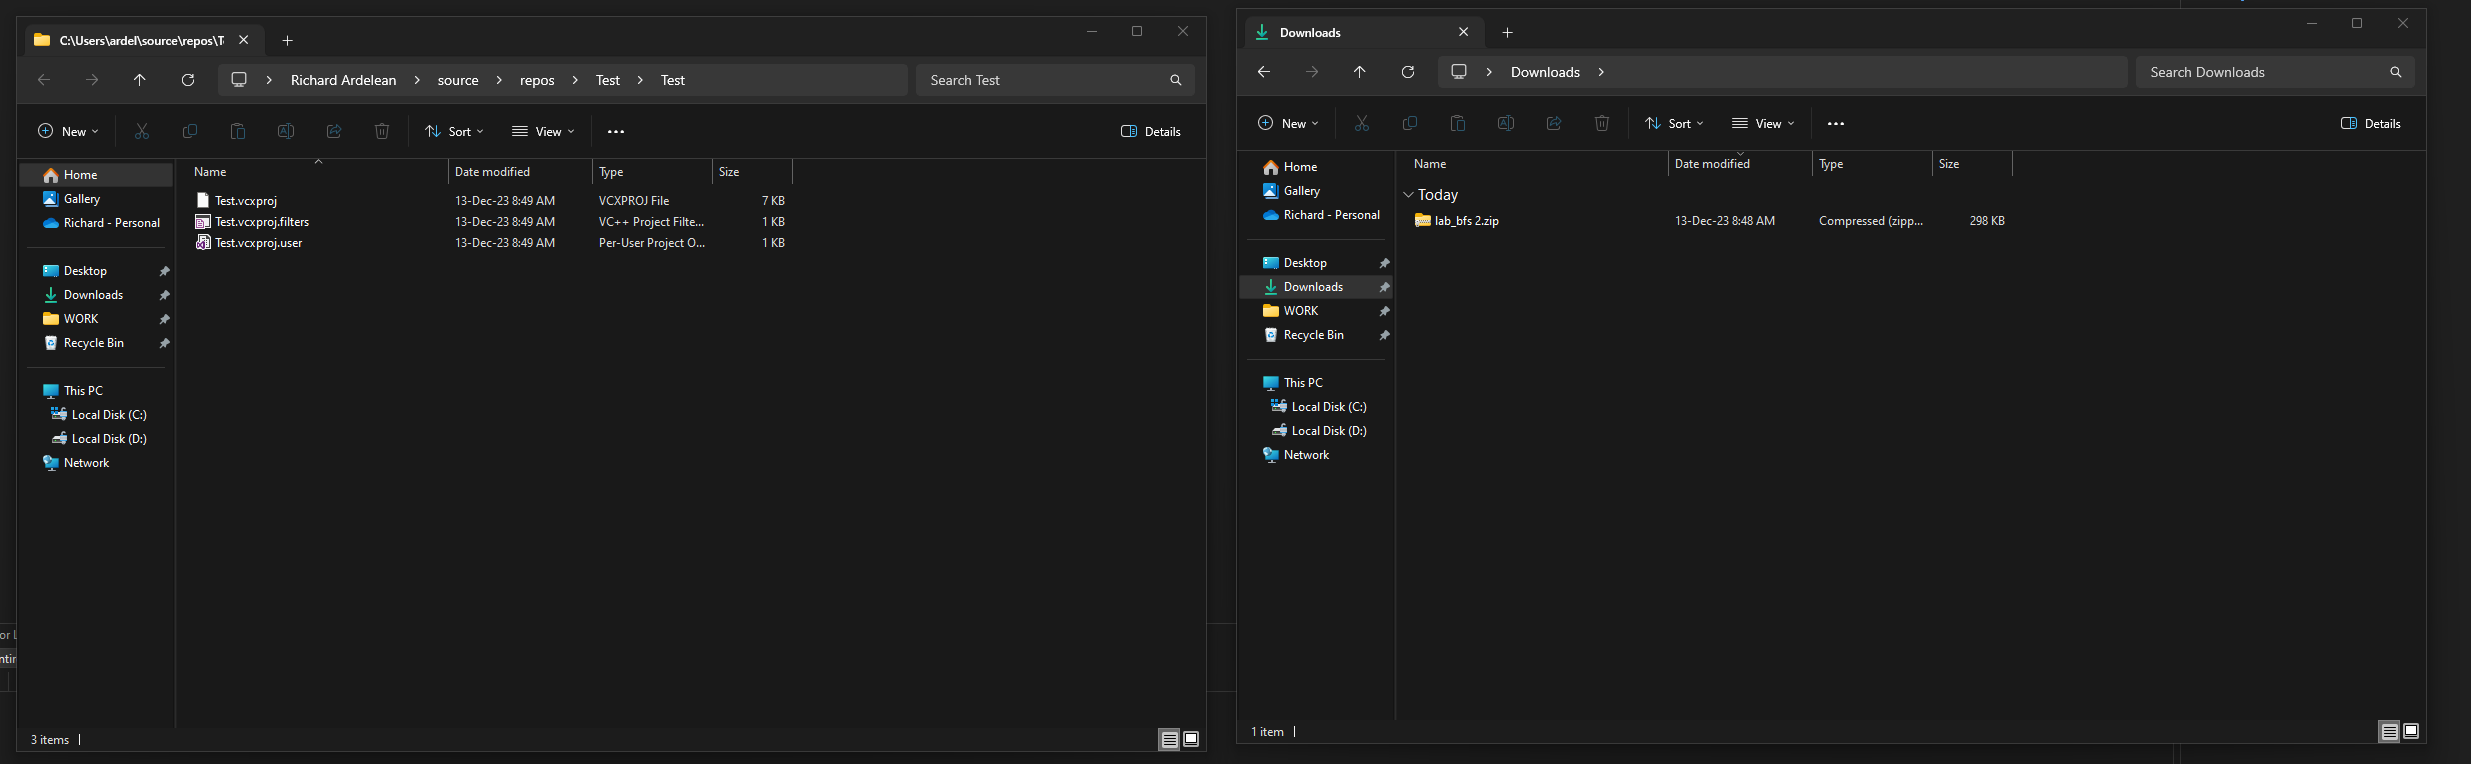
\includegraphics[width=\textwidth,alt={A screenshot of a computer Description automatically generated}]{./Resources/tutorial_lab9/image3.png}

\begin{enumerate}
\def\labelenumi{\arabic{enumi}.}
\setcounter{enumi}{3}
\item
  Deschideți fișierul `.zip' și copiați, așa cum se arată mai jos, fișierele din arhivă în folderul proiectului.
\end{enumerate}

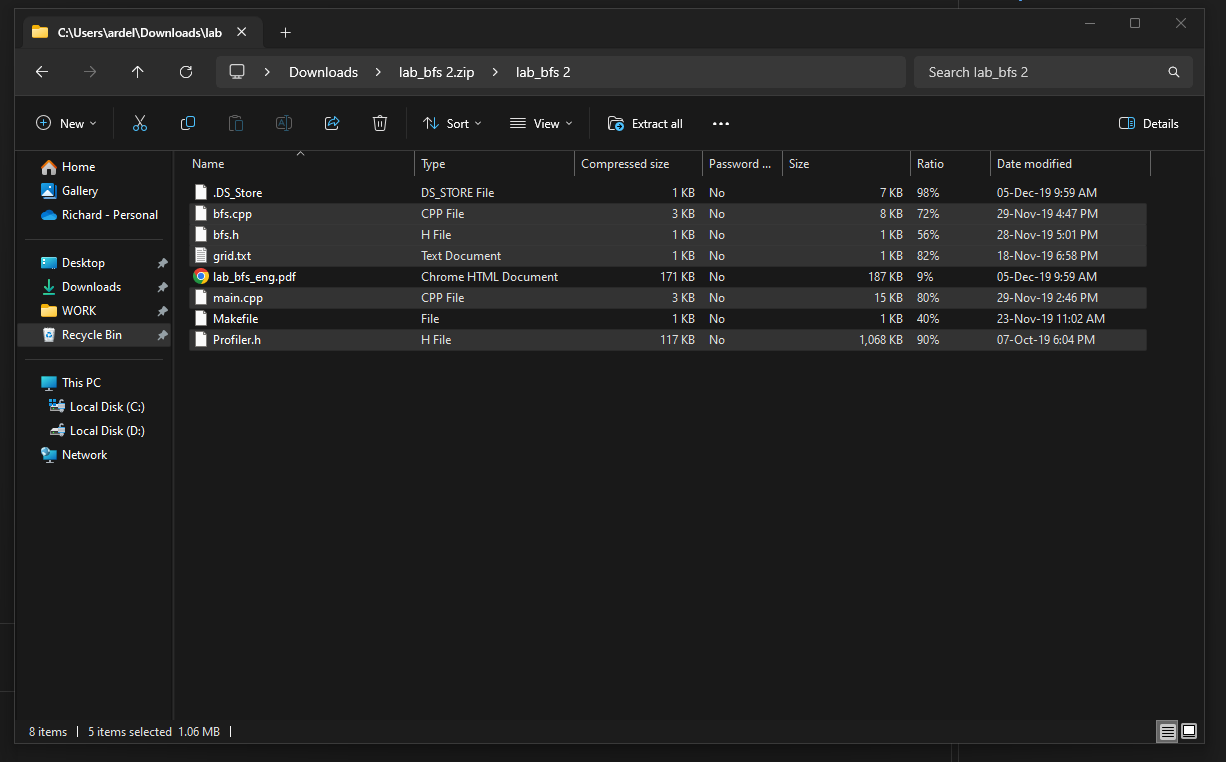
\includegraphics[width=\textwidth,alt={A screenshot of a computer Description automatically generated}]{./Resources/tutorial_lab9/image4.png}

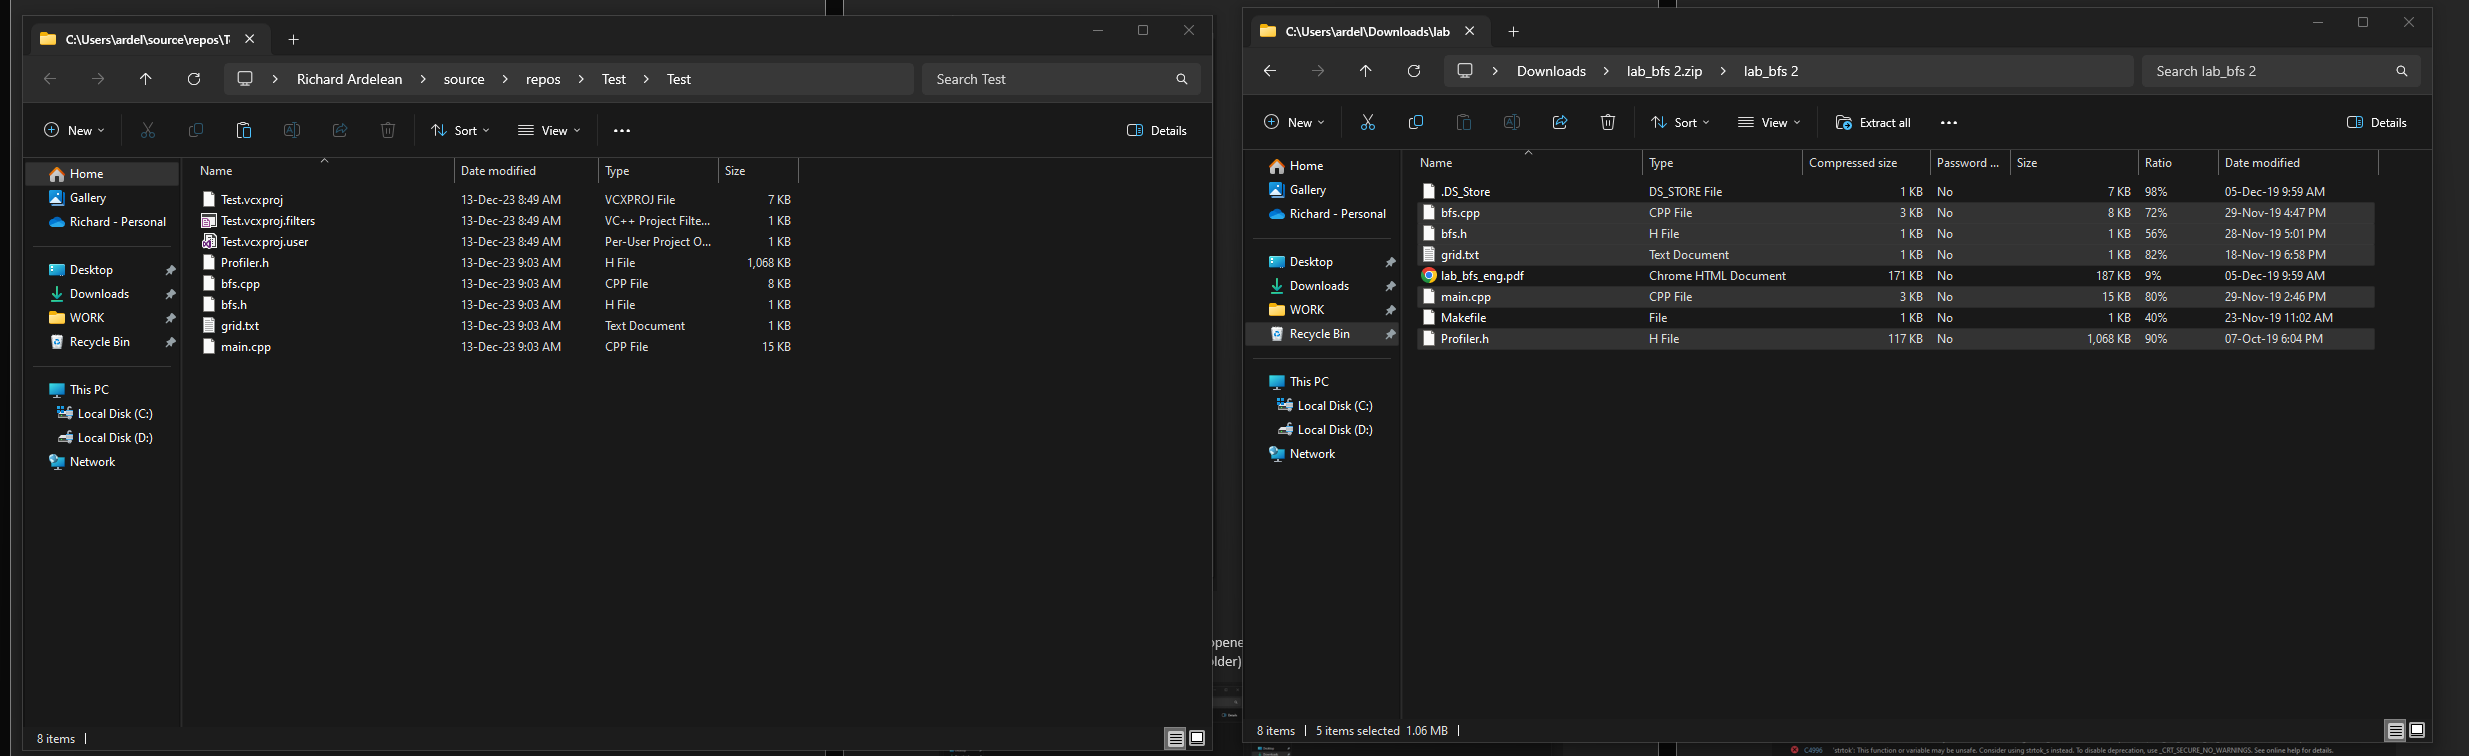
\includegraphics[width=\textwidth,alt={A screenshot of a computer Description automatically generated}]{./Resources/tutorial_lab9/image5.png}

\begin{enumerate}
\def\labelenumi{\arabic{enumi}.}
\setcounter{enumi}{4}
\item
  Selectând folderele din Solution Explorer al Visual Studio `Fișiere Header / Resurse / Fișiere Sursă` utilizați următoarele opțiuni:
\end{enumerate}

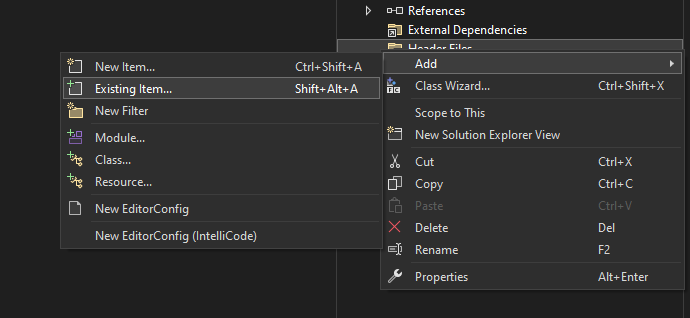
\includegraphics[width=\textwidth,alt={A screenshot of a computer Description automatically generated}]{./Resources/tutorial_lab9/image6.png}

\begin{enumerate}
\def\labelenumi{\arabic{enumi}.}
\setcounter{enumi}{5}
\item
  Astfel, se realizează următoarea structură:
\end{enumerate}

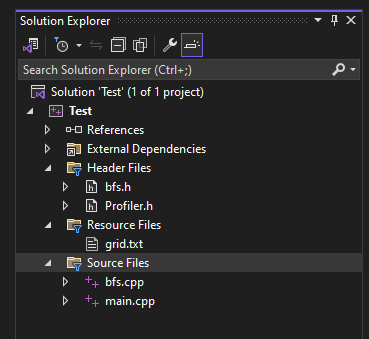
\includegraphics[width=\textwidth,alt={A screenshot of a computer Description automatically generated}]{./Resources/tutorial_lab9/image7.png}

\subsection{Eroare `unsafe' în Visual Studio}\label{visual-studio-unsafe-error}

Exemplu:

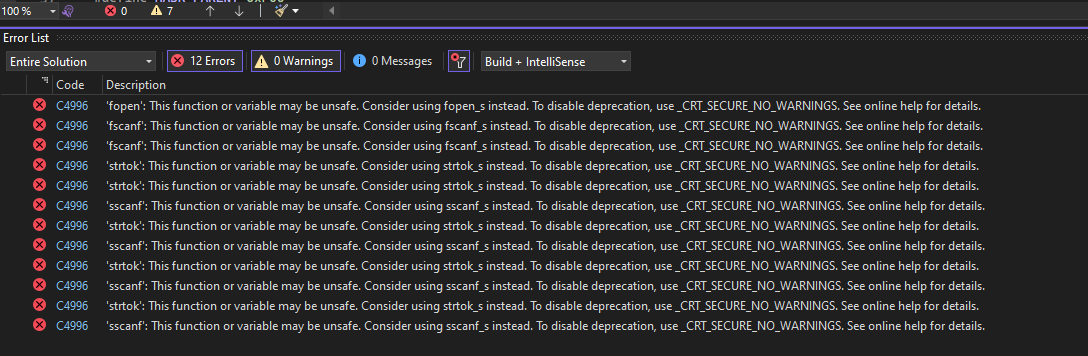
\includegraphics[width=\textwidth,alt={A screenshot of a computer Description automatically generated}]{./Resources/tutorial_lab9/image8.png}

Soluție:

Faceți clic dreapta pe proiect (nu pe Soluție, care cel mai probabil are același nume) și selectați `Proprietăți`.

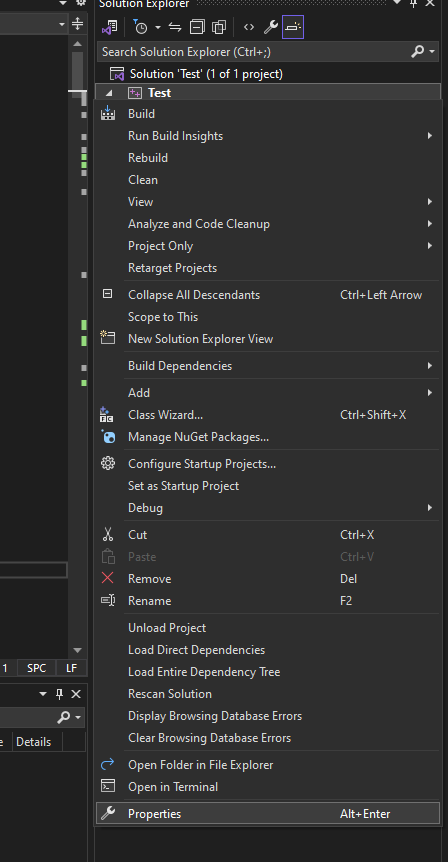
\includegraphics[width=\textwidth,alt={A screenshot of a computer program Description automatically generated}]{./Resources/tutorial_lab9/image9.png}

Actualizați `Configurație` și `Platformă` în partea superioară a ferestrei la `Toate configurațiile` și `Toate platformele`, respectiv.

Mergeți la `C/C++` și selectați `Preprocesor`.

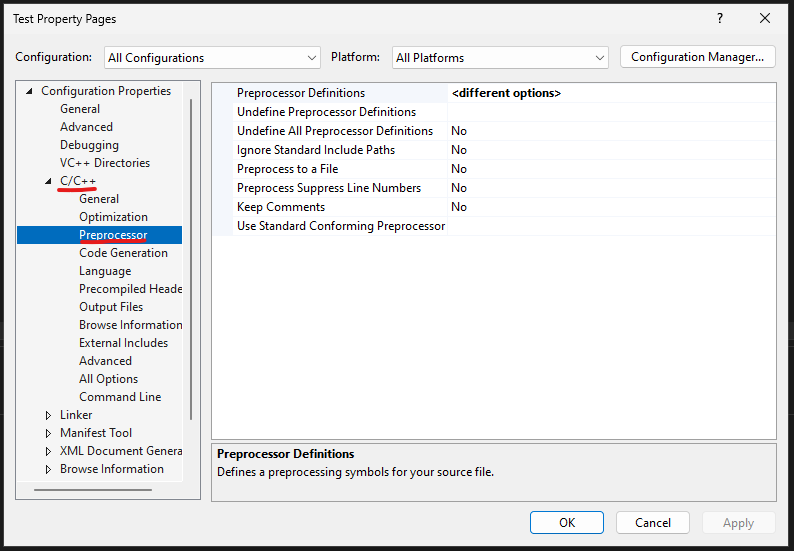
\includegraphics[width=\textwidth,alt={A screenshot of a computer Description automatically generated}]{./Resources/tutorial_lab9/image10.png}

Apoi faceți clic pe `Definiții Preprocesor` și pe săgeata dropdown.

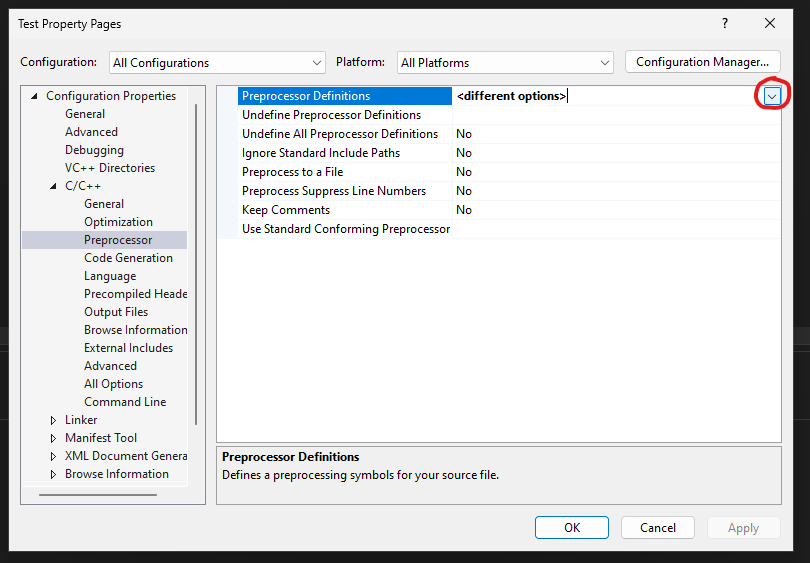
\includegraphics[width=\textwidth,alt={A screenshot of a computer Description automatically generated}]{./Resources/tutorial_lab9/image11.png}

Selectați `Editare`

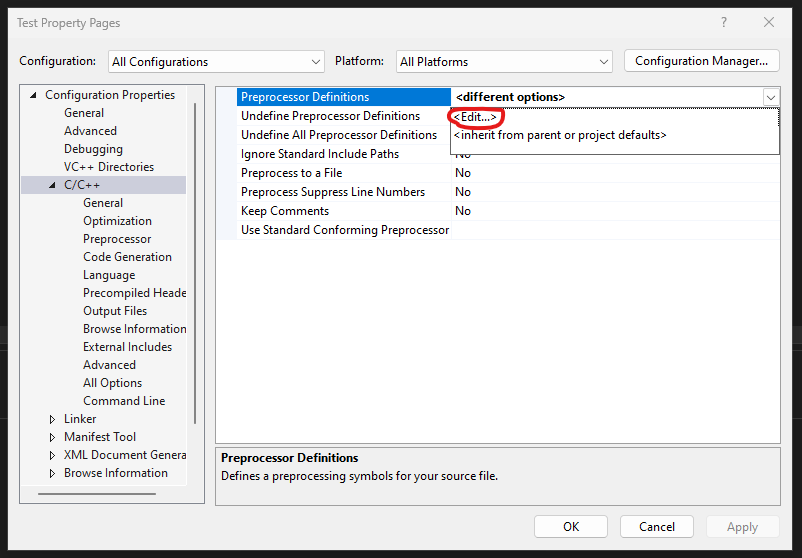
\includegraphics[width=\textwidth,alt={A screenshot of a computer Description automatically generated}]{./Resources/tutorial_lab9/image12.png}

Și se va deschide următoarea fereastră nouă:

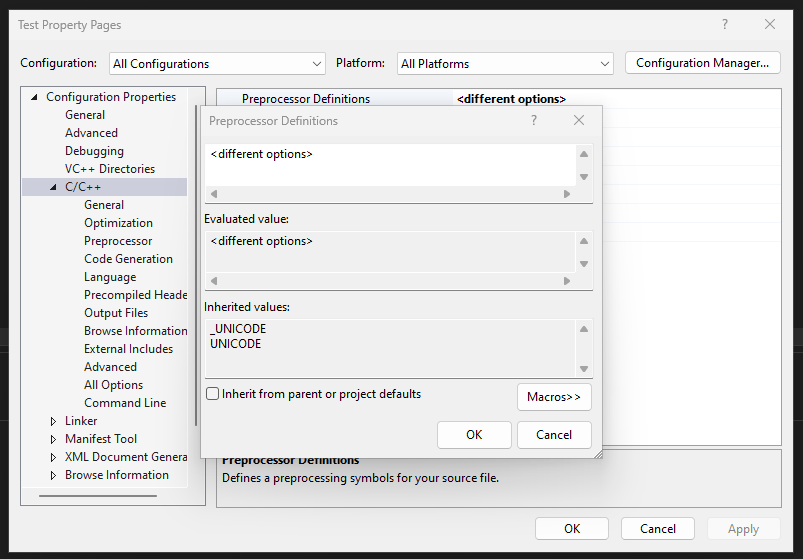
\includegraphics[width=\textwidth,alt={A screenshot of a computer Description automatically generated}]{./Resources/tutorial_lab9/image13.png}

Introduceți `\_CRT\_SECURE\_NO\_WARNINGS` sub `\textless opțiuni diferite\textgreater`, așa cum se arată mai jos.

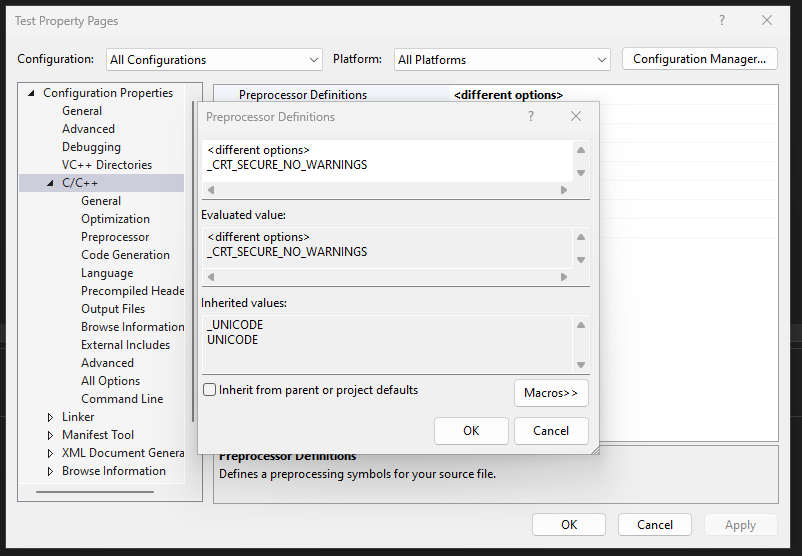
\includegraphics[width=\textwidth,alt={A screenshot of a computer Description automatically generated}]{./Resources/tutorial_lab9/image14.png}

Faceți clic pe `OK` la toate ferestrele deschise până când reveniți la fereastra principală Visual Studio a proiectului și veți putea rula proiectul.

\subsection{Eroare `Assertion` în Visual Studio}\label{visual-studio-assertion-error}

Aceasta indică faptul că nu ați urmat tutorialul. Întoarceți-vă la prima pagină și asigurați-vă că ați mutat fișierele din folderul `Downloads` în folderul `Project`. De asemenea, este posibil să fie nevoie să \emph{ștergeți} toate fișierele din IDE-ul Visual Studio și să le \emph{adăugați din nou} manual.

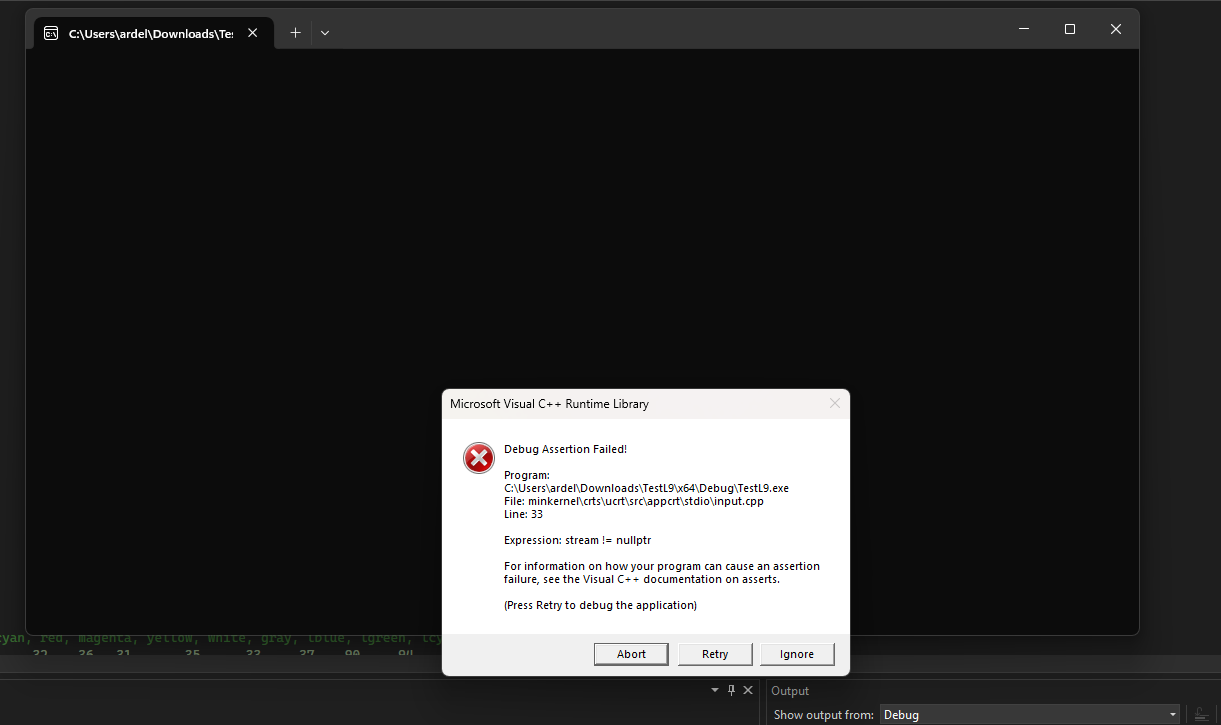
\includegraphics[width=\textwidth,alt={A screenshot of a computer Description automatically generated}]{./Resources/tutorial_lab9/image15.png}

\subsection{Eroare undefined în CLion}\label{clion-undefined-error}

Exemplu:

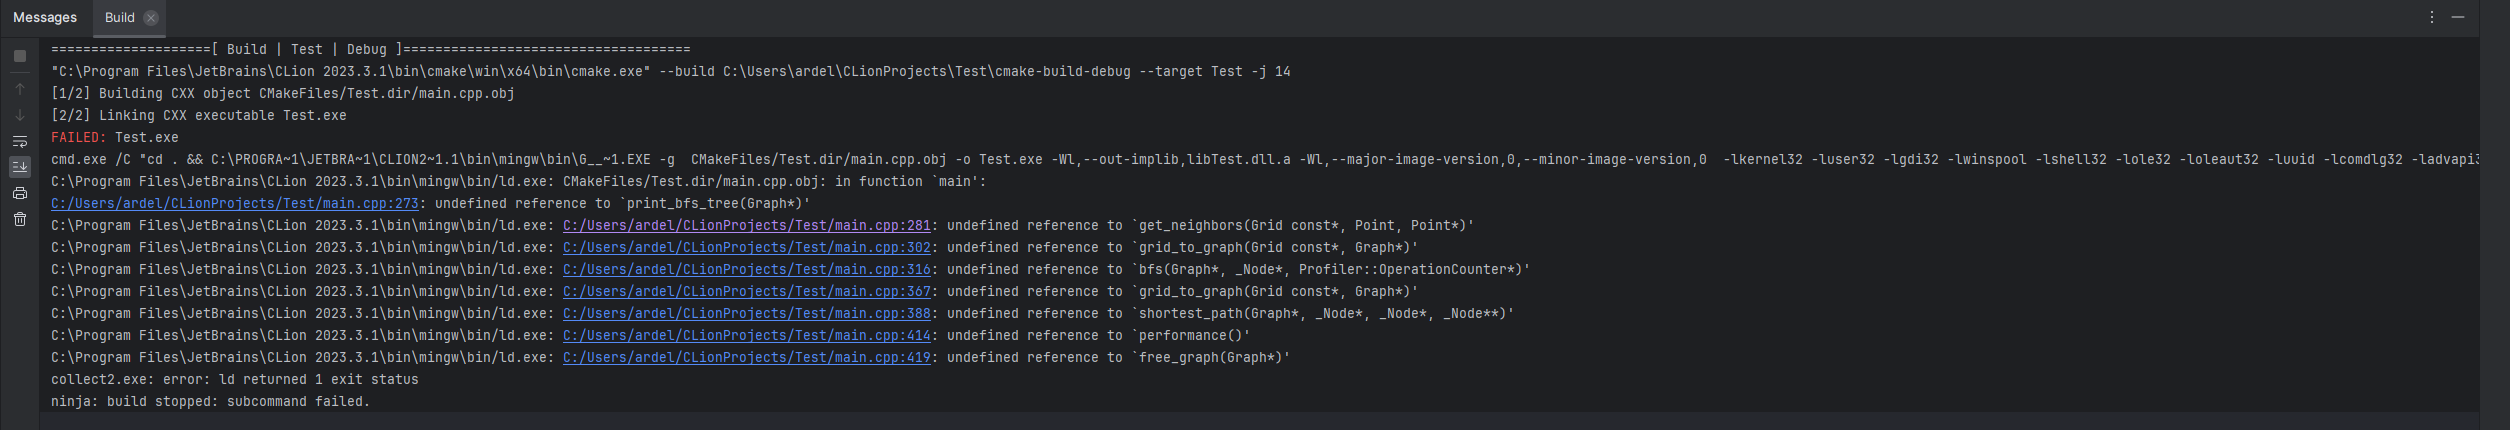
\includegraphics[width=\textwidth,alt={A screen shot of a computer Description automatically generated}]{./Resources/tutorial_lab9/image16.png}

Soluție:

Deschideți fișierul `CMakeLists.txt` și modificați după cum urmează:

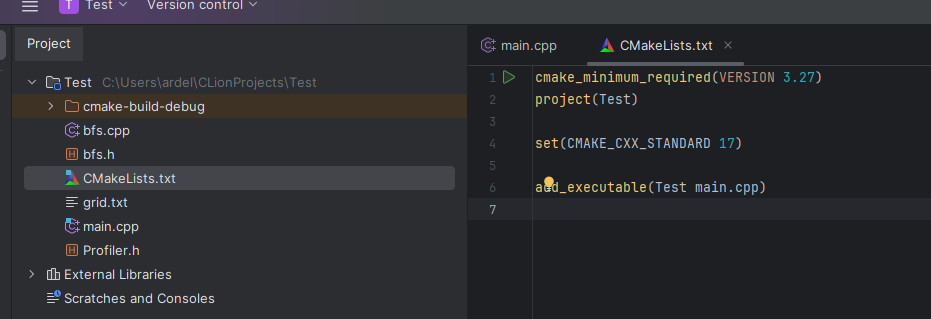
\includegraphics[width=\textwidth,alt={A screenshot of a computer Description automatically generated}]{./Resources/tutorial_lab9/image17.png}

adăugați

\begin{verbatim}
add_executable(Test main.cpp)
\end{verbatim}

în

\begin{verbatim}
add_executable(Test main.cpp bfs.cpp)
\end{verbatim}

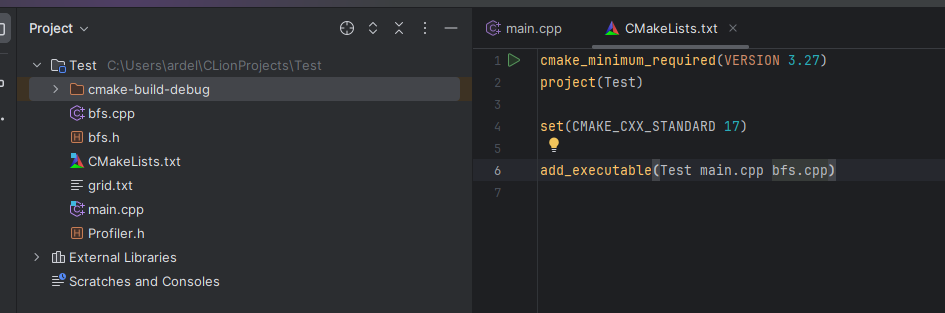
\includegraphics[width=\textwidth,alt={A screenshot of a computer Description automatically generated}]{./Resources/tutorial_lab9/image18.png}

\subsection{CLion Visual Studio – Opțiunea 1 (mai lentă)}\label{clion-visual-studio-option-1-slower}

Mergeți la `Fișier` -> `Setări`:

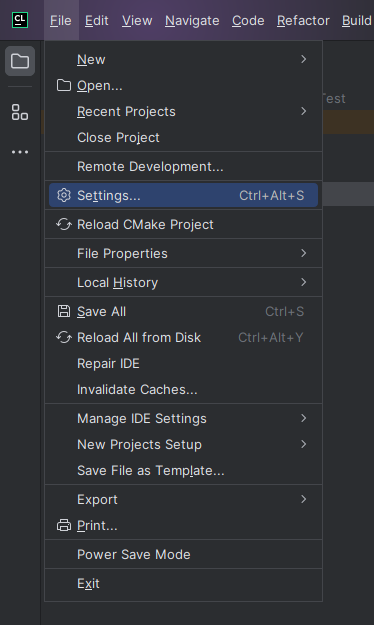
\includegraphics[width=\textwidth,alt={A screenshot of a computer program Description automatically generated}]{./Resources/tutorial_lab9/image19.png}

În fereastra nou deschisă, mergeți la `Compilare, Execuție, Implementare` -> `Lanțuri de instrumente`

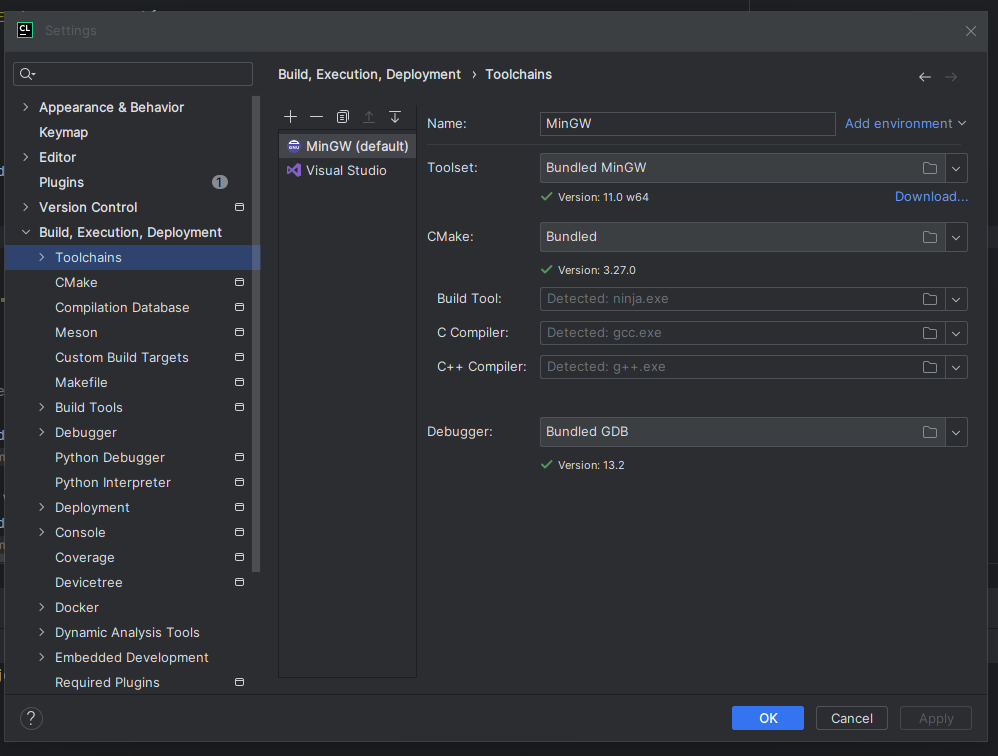
\includegraphics[width=\textwidth,alt={A screenshot of a computer Description automatically generated}]{./Resources/tutorial_lab9/image20.png}

Folosind săgețile, setați Visual Studio ca implicit:

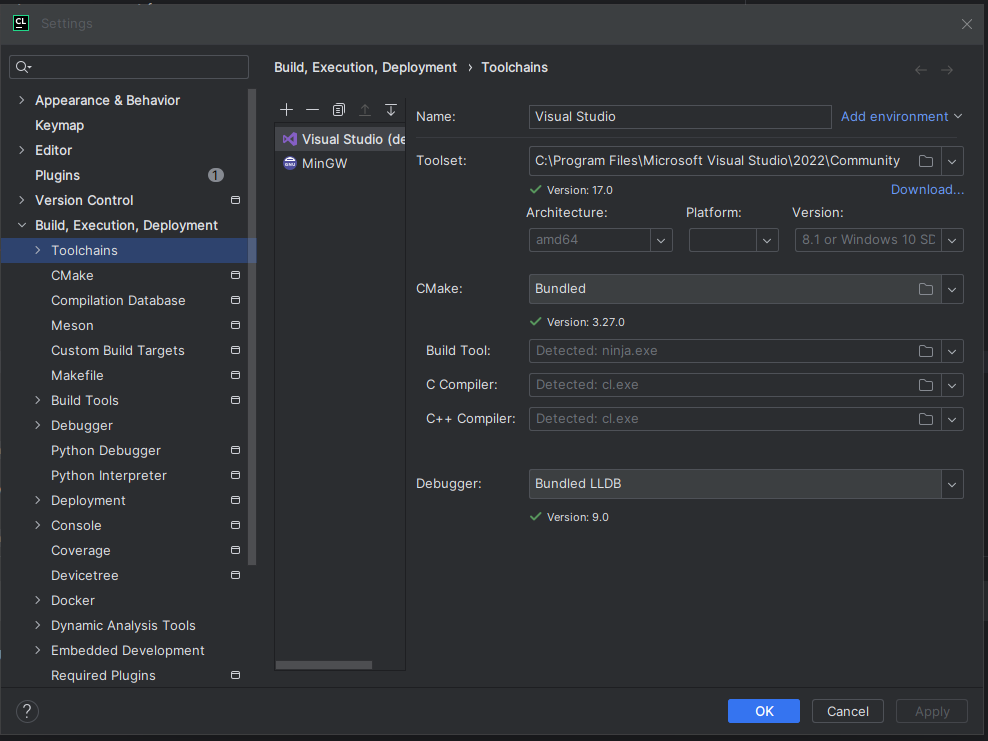
\includegraphics[width=\textwidth,alt={A screenshot of a computer Description automatically generated}]{./Resources/tutorial_lab9/image21.png}

\subsection{CLion MinGW – Opțiunea 2 (mai rapidă, necesită consolă externă)}\label{clion-mingw-option-2-faster-requires-external-console}

\subsubsection{Eroare Clear în CLion}\label{clion-clear-error}

Exemplu:

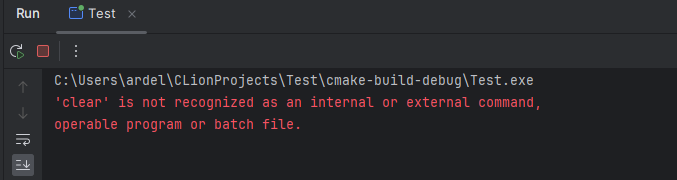
\includegraphics[width=\textwidth,alt={A screenshot of a computer program Description automatically generated}]{./Resources/tutorial_lab9/image22.png}

Soluție:

Accesați fișierul main.cpp și derulați la liniile 113-117 în funcția displayGrid.

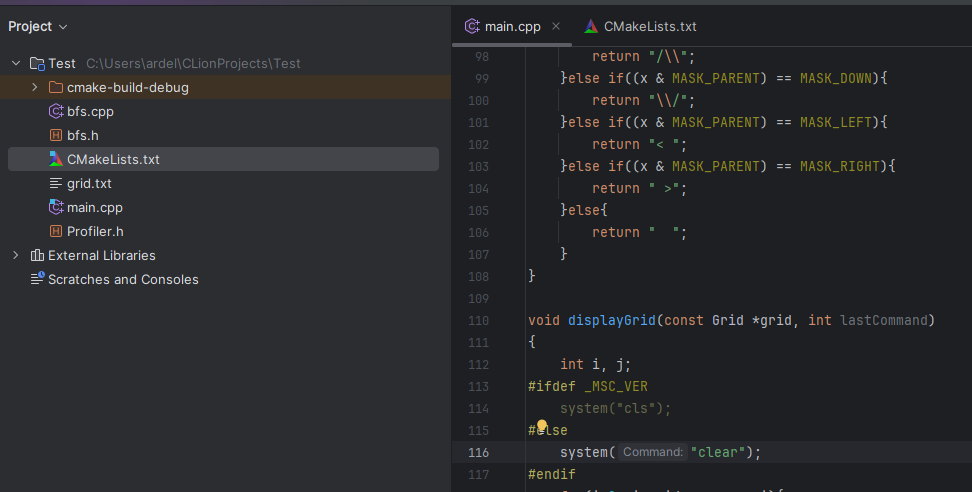
\includegraphics[width=\textwidth,alt={A screen shot of a computer Description automatically generated}]{./Resources/tutorial_lab9/image23.png}

Modificați după cum urmează:

În ramura else de la linia 116

\begin{verbatim}
system("clear");
\end{verbatim}

înlocuiți cu

\begin{verbatim}
system("cls");
\end{verbatim}

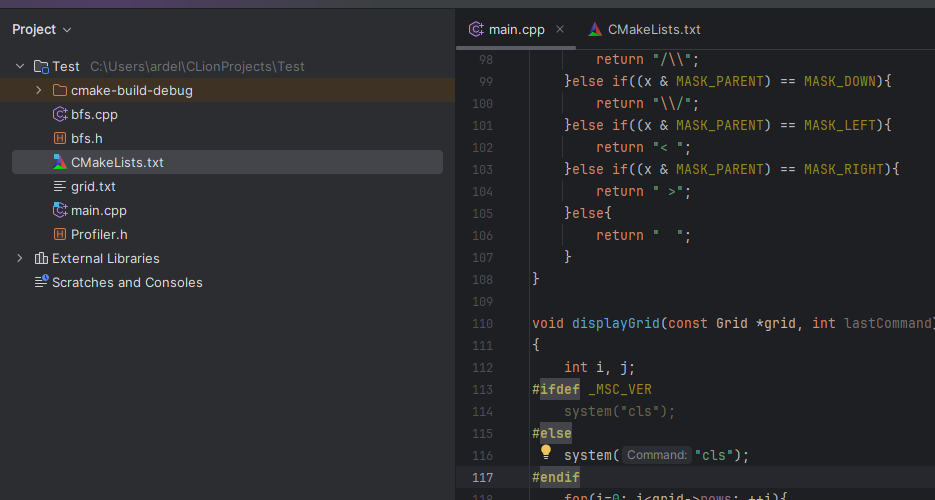
\includegraphics[width=\textwidth,alt={A screenshot of a computer program Description automatically generated}]{./Resources/tutorial_lab9/image24.png}

\subsubsection{CLion nu afișează grila}\label{clion-not-showing-grid}

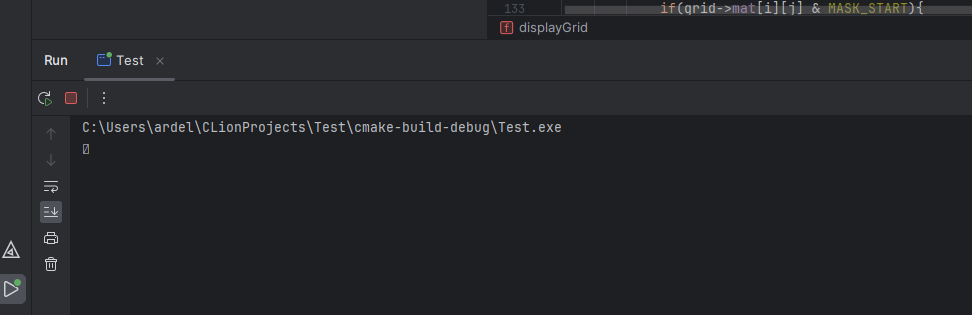
\includegraphics[width=\textwidth,alt={A screenshot of a computer Description automatically generated}]{./Resources/tutorial_lab9/image25.png}

Copiați fișierul `grid.txt` în folderul `cmake-build-debug`.

Apoi, mergeți în partea dreaptă sus a ecranului:

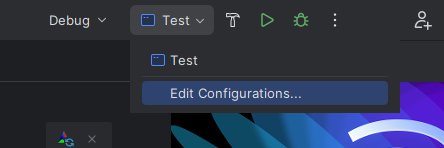
\includegraphics[width=\textwidth,alt={A screenshot of a computer Description automatically generated}]{./Resources/tutorial_lab9/image26.png}

Selectați `Edit Configurations` și bifați următoarele opțiuni:

\begin{itemize}
\item
  Rulați în consolă externă
\end{itemize}

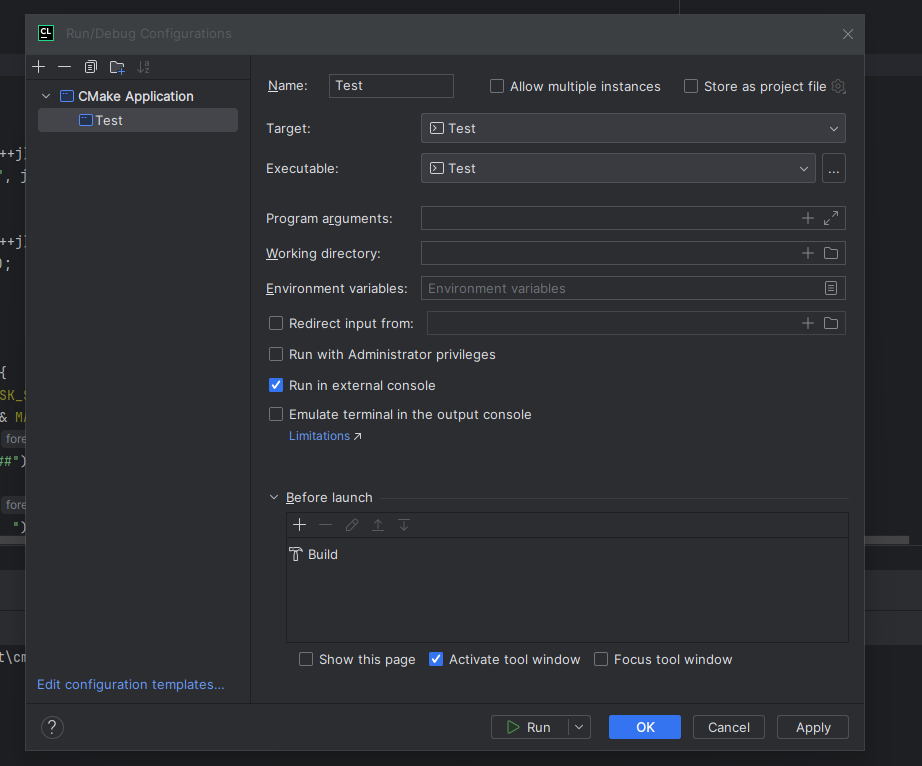
\includegraphics[width=\textwidth,alt={A screenshot of a computer Description automatically generated}]{./Resources/tutorial_lab9/image27.png}

\subsection{Comanda de rulare pe Mac}\label{mac-run-command}

\begin{verbatim}
g++ main.cpp bfs.cpp -std=c++11 && ./a.out
\end{verbatim}


\end{document}
